\documentclass[twocolumn,10pt]{article}
\usepackage[letterpaper,left=1.95cm,right=1.95cm,top=2.5cm,bottom=3.16cm]{geometry}
\usepackage{natbib}
\usepackage{hyperref}
\usepackage{enumitem}
\usepackage{balance}
\usepackage{booktabs}
\usepackage{graphicx}
\usepackage{amsmath}
\usepackage{amssymb}
\usepackage[utf8]{inputenc}
\usepackage{wasysym} % symbols
\usepackage{amssymb} % symbols
\usepackage{abstract}
\usepackage{parskip}
\usepackage{hyperref}
\usepackage{titlesec}
\usepackage{xcolor}
\usepackage{natbib}
\usepackage{float}
\usepackage{graphicx}
\usepackage{fancyhdr}
\usepackage{titling}
\usepackage{caption}
\usepackage[document]{ragged2e}
\usepackage[affil-sl]{authblk} 
\usepackage{mathptmx}  %Times new Roman

\setlength{\columnsep}{1cm}
\renewcommand{\refname}{BIBLIOGRAFÍA}
\renewcommand{\figurename}{Fig.}
\renewcommand{\tablename}{Tabla.}
\renewcommand{\abstractname}{RESUMEN}

% Keywords command
\providecommand{\keywordsSpan}[1]
{
  \small	
  \textbf{\textit{Palabras Clave:}} #1
}

\providecommand{\keywordsEng}[1]
{
  \small	
  \textbf{\textit{Keywords:}} #1
}


%%%%%%%% FORMATO DE LAS SECCIONES Y SUBSECCIONES %%%%%
\titleformat{\section} 
	{\normalfont\large\bfseries}{\makebox[30pt][l]{\thesection}}{0pt}{} 
\titleformat{\subsection} 
	{\normalfont\large\bfseries }{\makebox[30pt][l]{\thesubsection}}{0pt}{}
\renewcommand\thesection{\arabic{section}.}
\renewcommand\thesubsection{\thesection\arabic{subsection}}
%%%%%%%% FORMATO DE LAS SECCIONES Y SUBSECCIONES %%%%%


	
\makeatletter
\long\def\@makecaption#1#2{
\vskip\abovecaptionskip
\sbox\@tempboxa{#1. #2}
\ifdim \wd\@tempboxa >\hsize
#1. #2\par
\else
\global \@minipagefalse
\hb@xt@\hsize{\hfil\box\@tempboxa\hfil}
\fi
\vskip\belowcaptionskip}
\makeatother


\pagestyle{fancyplain}% <- pagestyle fancyplain

\fancyfoot[C]{}
\renewcommand\plainheadrulewidth{.4pt}% headrule on plain pages
%\fancyhf{}
\rhead{Semestre 4 Año 2026}
\lhead{Estadística Bayesiana}
\rfoot{\thepage}

\date{}
 

%%%%%%% ENCABEZADO %%%%%%%%%%%%%%%%%%%%

{\title{\fontsize{16}{16}\selectfont
\vspace*{-0.7cm}
\textbf{
Entrega 02: Diseño Metodológico y EDA - Proyecto CS:GO
} \\[0.2cm]
\fontsize{12}{12}\selectfont
\textbf{Predicting the Unpredictable: A Bayesian Statistics Approach to Estimate Win Probability in CS:GO}\\[0.2cm]}
}

\author[1,*]{\fontsize{10pt}{10pt}\selectfont \textbf{Julián Duarte}}
\author[2]{\textbf{Julián Jiménez}}
\author[3]{\textbf{Tomás Rincón}}

\affil[1]{\fontsize{8pt}{8pt}\selectfont Pregrado Ciencia de Datos Universidad Externado, Bogotá - Colombia}
\affil[2]{Pregrado Ciencia de Datos Universidad Externado, Bogotá - Colombia}
\affil[3]{Pregrado Ciencia de Datos Universidad Externado, Bogotá - Colombia \vspace{0.2cm}} 
\affil[*]{julian.duarte2@est.uexternado.edu.co; julian.jimenez5@est.uexternado.edu.co; juan.rincon14@est.uexternado.edu.co}

\begin{document}

\twocolumn[
  \begin{@twocolumnfalse}
    \maketitle

    \begin{center}
        \textbf{RESUMEN}
    \end{center}
    Este documento presenta el diseño metodológico y el análisis exploratorio de datos (EDA) para el proyecto de estimación de probabilidad de victoria en CS:GO mediante estadística bayesiana. Se profundiza en la fundamentación teórica, se definen las estrategias de modelado y se presentan los hallazgos iniciales de la estructura de datos, permitiendo una cuantificación explícita de la incertidumbre en un entorno competitivo de alta volatilidad.
    \vspace{0.2cm}

    \keywordsSpan{Esports, Estadística Bayesiana, CS:GO, Diseño Metodológico, EDA, Incertidumbre.}
    
    \vspace{0.6cm}
  \end{@twocolumnfalse}
]

\thispagestyle{fancyplain}

\section{PROFUNDIZACIÓN DE LA ENTREGA 1}

\subsection{Problema y Pregunta de Investigación Refinados}
El ecosistema competitivo de CS:GO/CS2 demanda herramientas de análisis de riesgo capaces de gestionar la incertidumbre. Los modelos tradicionales suelen fallar al ignorar la naturaleza estocástica del juego, centrándose únicamente en si un equipo gana o pierde sin cuantificar el margen de error. Nuestra investigación se centra en capturar esta complejidad.

\textbf{Pregunta de investigación:} ¿De qué manera influyen la destreza técnica de los equipos y las ventajas tácticas del mapa en la probabilidad de victoria en CS:GO, y cómo podemos medir qué tan seguros estamos de estos pronósticos ante la naturaleza impredecible del juego?

\subsection{Revisión de Literatura Fortalecida}
Se ha identificado un vacío crítico en la calibración probabilística de los modelos actuales de Esports. Mientras que la mayoría se enfoca en el \textit{accuracy} (precisión cruda), nuestro enfoque prioriza la gestión del riesgo mediante métricas especializadas:

\begin{itemize}
    \item \textbf{Brier Score:} Esta métrica es fundamental para evaluar qué tan \textit{calibradas} están nuestras probabilidades. A diferencia de la precisión simple, el Brier Score mide la distancia cuadrática entre la probabilidad asignada y el resultado real, castigando la sobreconfianza en pronósticos erróneos. Un modelo con un buen Brier Score es aquel que no solo acierta, sino que asigna probabilidades realistas a sus aciertos y fallos.
    \item \textbf{HDI (Highest Density Interval):} En el paradigma bayesiano, el HDI representa el intervalo de la distribución posterior que contiene los valores más probables (por ejemplo, el 95\% de la masa de probabilidad). A diferencia de los intervalos de confianza tradicionales, el HDI nos permite decir con rigor científico en qué rango se encuentra la verdadera probabilidad de victoria, ofreciendo una medida directa de la incertidumbre o "seguridad" del modelo ante cada partida.
\end{itemize}

\section{SECCIÓN DE METODOLOGÍA}

\subsection{Enfoque del Estudio}
El estudio adopta un enfoque confirmatorio y predictivo bajo el paradigma bayesiano. Se utiliza un modelo paramétrico que permite integrar conocimiento experto mediante distribuciones \textit{prior}.

\subsection{Datos}
Se utiliza el dataset consolidado \texttt{csgo\_games.csv}, el cual integra métricas avanzadas de \textit{HLTV.org} de más de 3,700 enfrentamientos profesionales. Este dataset es fundamental ya que nos permite acceder a los ratings e impactos individuales de cada jugador por equipo, permitiendo una granularidad superior en la definición de las \textit{priors} del modelo.

\subsection{Estrategia Metodológica}
La estrategia consiste en:
\begin{enumerate}
    \item Procesamiento y normalización de variables relativas.
    \item Definición de \textit{priors} basadas en el análisis descriptivo.
    \item Muestreo mediante el algoritmo NUTS (No-U-Turn Sampler).
    \item Validación mediante validación cruzada para series temporales.
\end{enumerate}

\subsection{Elección y Justificación del Modelo}
Se ha seleccionado una \textbf{Regresión Logística Bayesiana Jerárquica}. La jerarquización permite el \textit{partial pooling}, mejorando las predicciones para equipos con pocos datos al aprender de la tendencia global del circuito.

\subsection{Limitaciones}
El modelo se limita a datos \textit{pre-match}. No considera cambios de alineación de último minuto ni factores psicológicos o ambientales que no estén registrados en las estadísticas oficiales.

\section{ANÁLISIS EXPLORATORIO DE DATOS (EDA)}

\subsection{Pregunta y Subpreguntas Analíticas}
\textbf{Pregunta central:} ¿Qué variables técnicas discriminan mejor entre victoria y derrota?
\begin{itemize}
    \item \textbf{S1:} ¿Cómo varía la probabilidad de victoria según el mapa seleccionado?
    \item \textbf{S2:} ¿Es el Diferencial de Rating un predictor más estable que el Diferencial de Impacto?
\end{itemize}

\subsection{Análisis Univariado y Bivariado}
Como se observa en la Figura \ref{fig:DistFig}, el diferencial de rating muestra una alta concentración cerca de cero, indicando una paridad extrema en la élite profesional.

\begin{figure}[h]
    \centering
    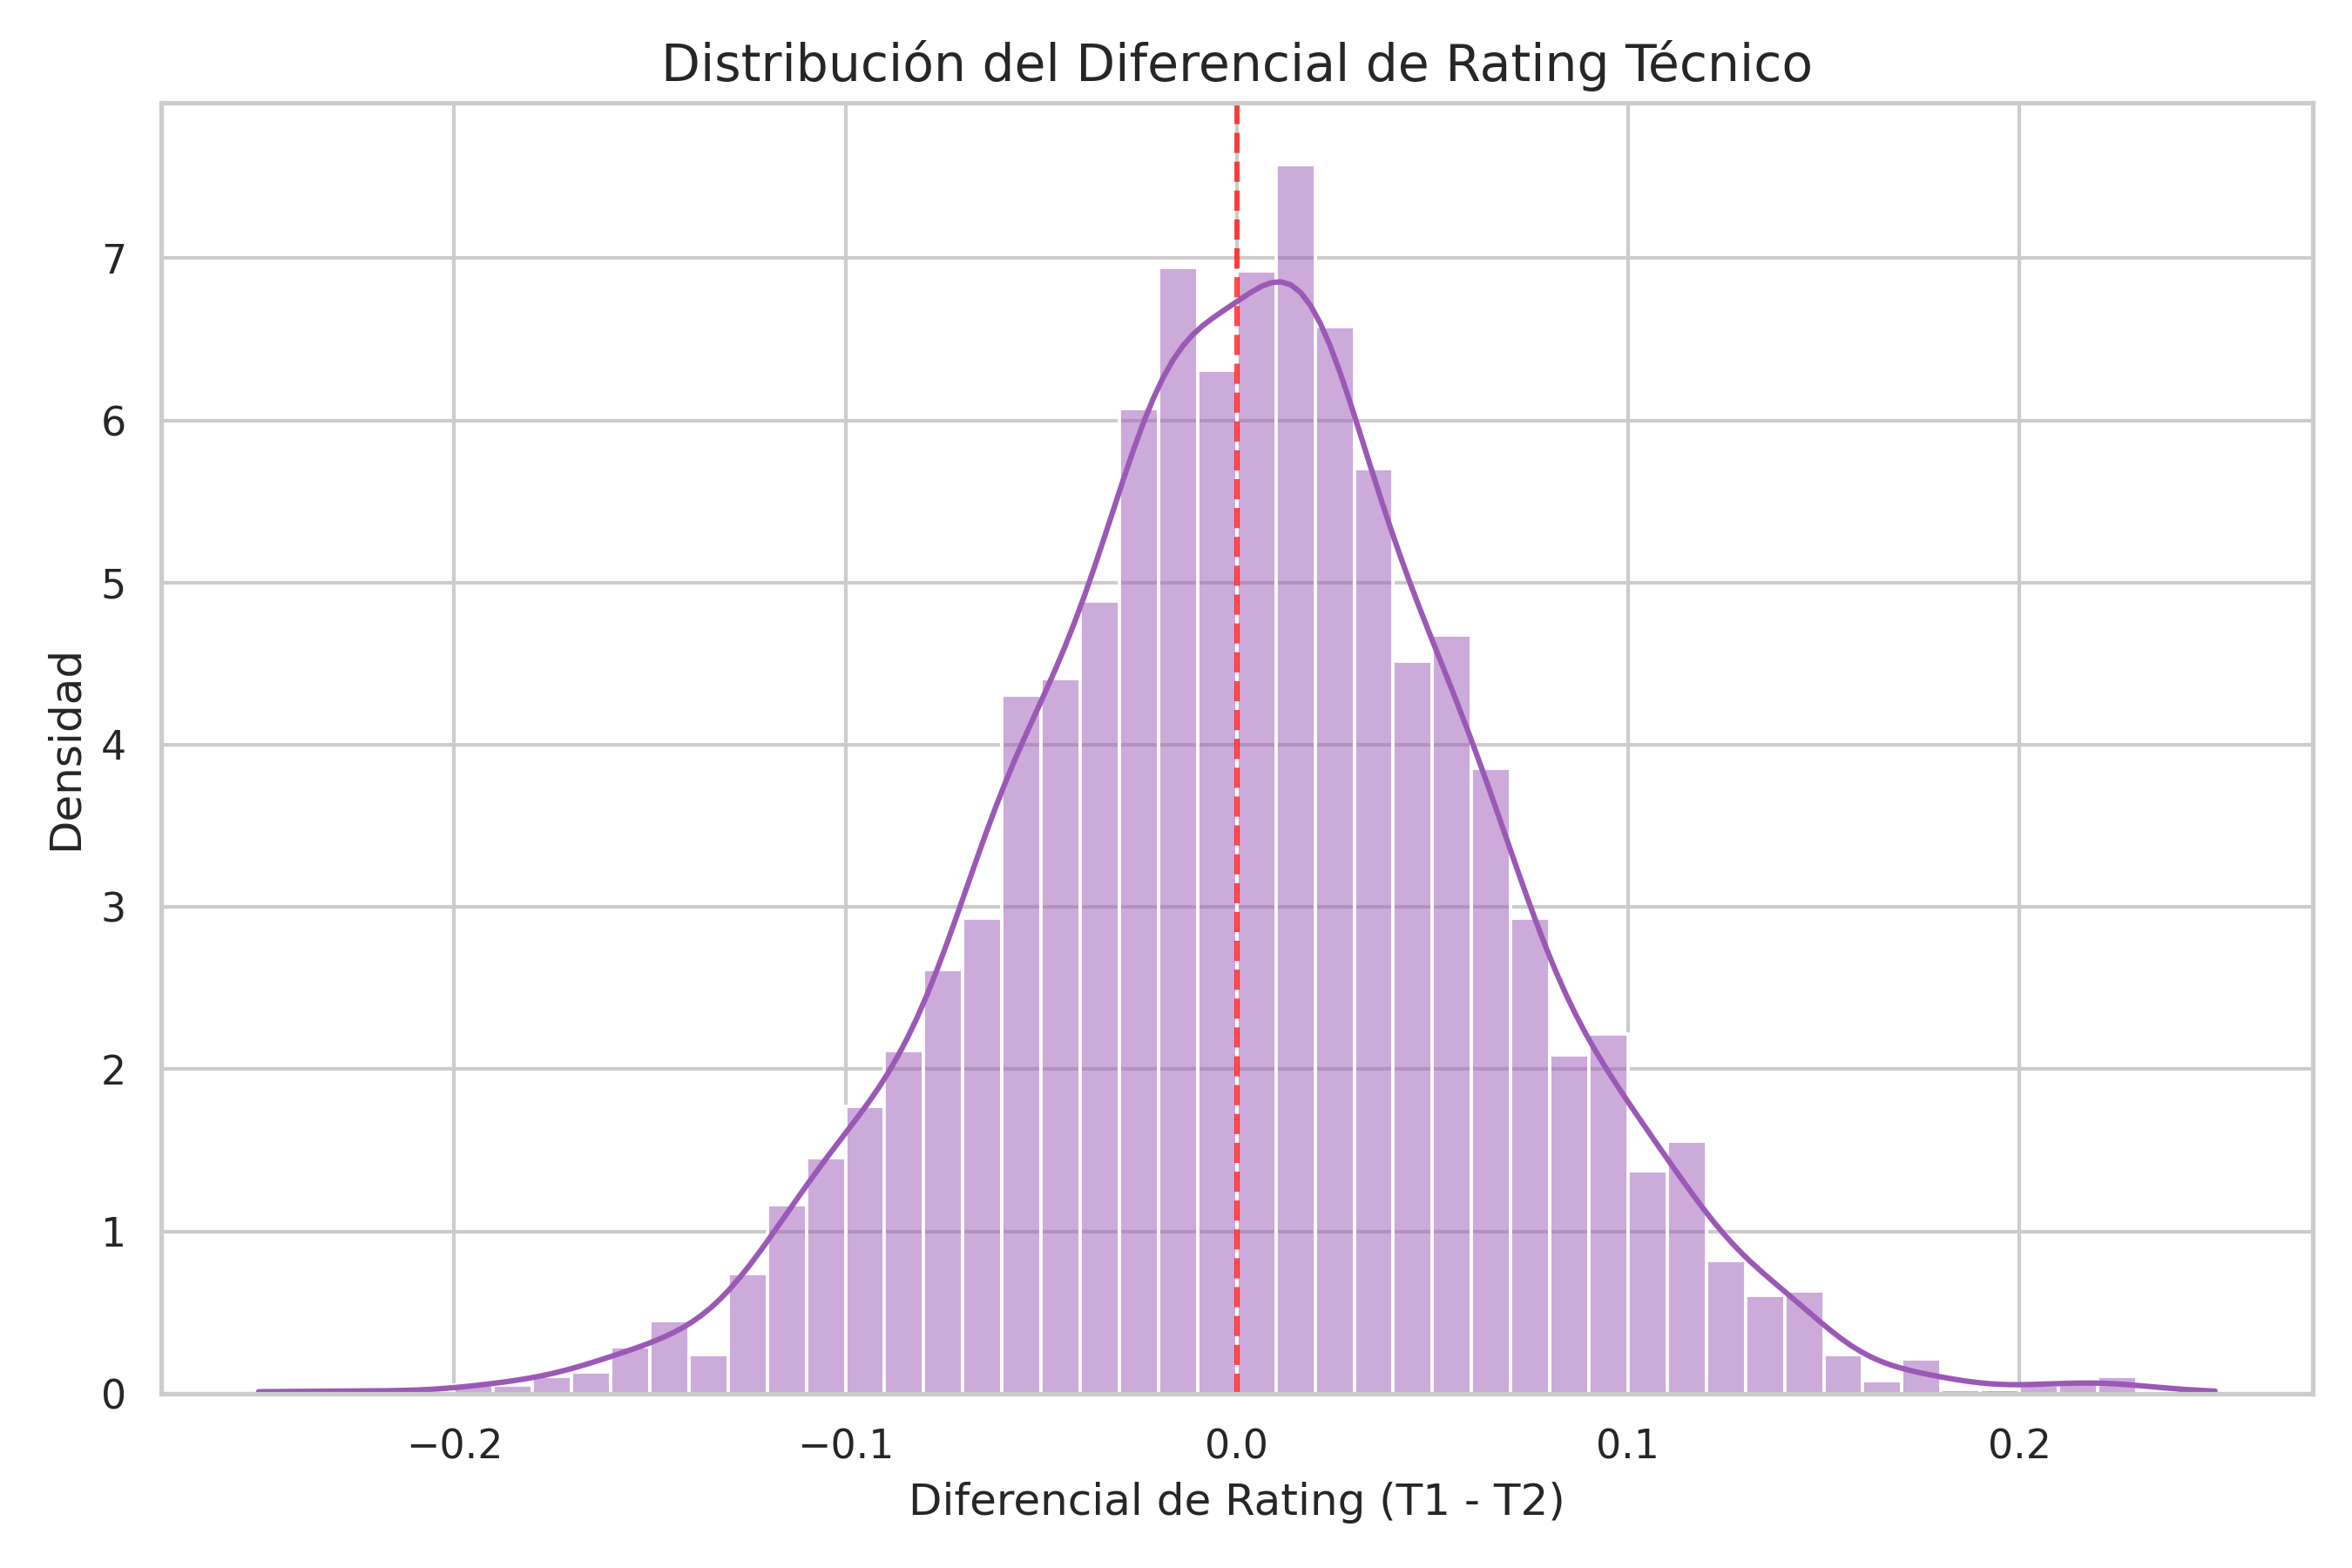
\includegraphics[width=\linewidth]{distribucion_densidad_rating.png}
    \caption{Distribución del Diferencial de Rating.}
    \label{fig:DistFig}
\end{figure}

\subsection{Resultados e Interpretación}
El análisis de correlación (Figura \ref{fig:CorrFig}) confirma que el Rating (0.26) y el Impacto táctico son los motores principales de la victoria.

\begin{figure}[h]
    \centering
    
\includegraphics[width=\linewidth]{matriz_correlacion_completa.png}
    \caption{Matriz de Correlación de variables clave.}
    \label{fig:CorrFig}
\end{figure}

\subsection{Implicaciones para el Modelo}
La alta volatilidad del impacto táctico sugiere que este debe modelarse con \textit{priors} más flexibles (mayor varianza), mientras que el Rating permite una regularización más estricta debido a su estabilidad.

\bibliographystyle{apalike}
\bibliography{bibliografia}

\end{document}
